\chapter{Measuring Higgs boson properties in the \Hgg decay channel}
\label{chap:hgg_overview}

\section{Introduction}
The following three chapters provide a detailed description of the CMS \Hgg analysis documented in Ref.~\cite{CMS-PAS-HIG-19-015}. This analysis measures Higgs boson properties in the diphoton decay channel, using proton-proton collision data at $\sqrt{s}$~=~13~TeV collected by the CMS experiment at the LHC from 2016 to 2018, corresponding to an integrated luminosity of 137~\fbinv. The increased statistical power, which comes with using the full Run 2 data, leads to an improvement in the precision of existing measurements and enables measurements of more granular regions of Higgs boson production phase space. 

Building upon the strategies developed in previous CMS \Hgg analyses~\cite{}, a set of orthogonal event categories are constructed to target bins at stage 1.2 of the STXS framework~\cite{}. The production cross sections are then measured directly from the diphoton invariant mass distributions in the event categories. This extremely powerful observable effectively distinguishes signal from background, where photon pairs produced via Higgs boson decay form a narrow signal peak centred around $m_H$, lying above a smoothly-falling background distribution from other SM processes. For events with two reconstructed photons, $\gamma_1$ and $\gamma_2$, the diphoton invariant mass, $m_{\gamma\gamma}$, is calculated according to,

\begin{equation}\label{eq:mgg}
    m_{\gamma\gamma} = \sqrt{2E_{\gamma1}E_{\gamma2}(1-\cos{\theta})},
\end{equation}

\noindent
where $E_{\gamma1}$ and $E_{\gamma2}$ are the measured energies of $\gamma_1$ and $\gamma_2$ respectively, and $\theta$ is the opening angle between the two photons. As displayed graphically in Figure~\ref{fig:hgg_overview_improving_measurements}, it is possible to isolate three aspects of the $m_{\gamma\gamma}$ spectrum which affect the sensitivity to Higgs boson properties: 

\begin{enumerate}
    \item The diphoton mass resolution: a narrower signal peak leads to enhanced sensitivity. This can be improved by correctly identifying photons from other objects in the detector such as jets, and subsequently making accurate measurements of the photon position and energy. Furthermore, the precise assertion of the interaction vertex from which the two photons originate is crucial for accurately determining the opening angle, $\theta$.
    
    \item The signal-to-background ratio in an event category: the sensitivity is improved by reducing the background contamination under the Higgs boson peak. In this analysis, traditional cut-based methods are improved upon by using machine learning algorithms, which better discriminate between signal and background. Since different background processes are important for different Higgs boson production modes, a number of signal-vs-background classifiers are trained and used in the relevant event categories.
    
    \item The purity of the signal events in an event category: here, event categories are defined to target specific bins of the STXS framework. Therefore to improve the sensitivity, we aim to maximise the purity of an event category with respect to the targeted bin. In other words, make the confusion matrix between the truth-level STXS bin and the reconstruction-level event category as diagonal as possible (see Figure~\ref{fig:purity_matrix}). This in turn reduces the correlations between the measured cross sections.
\end{enumerate}

\begin{figure}[hptb]
  \centering
  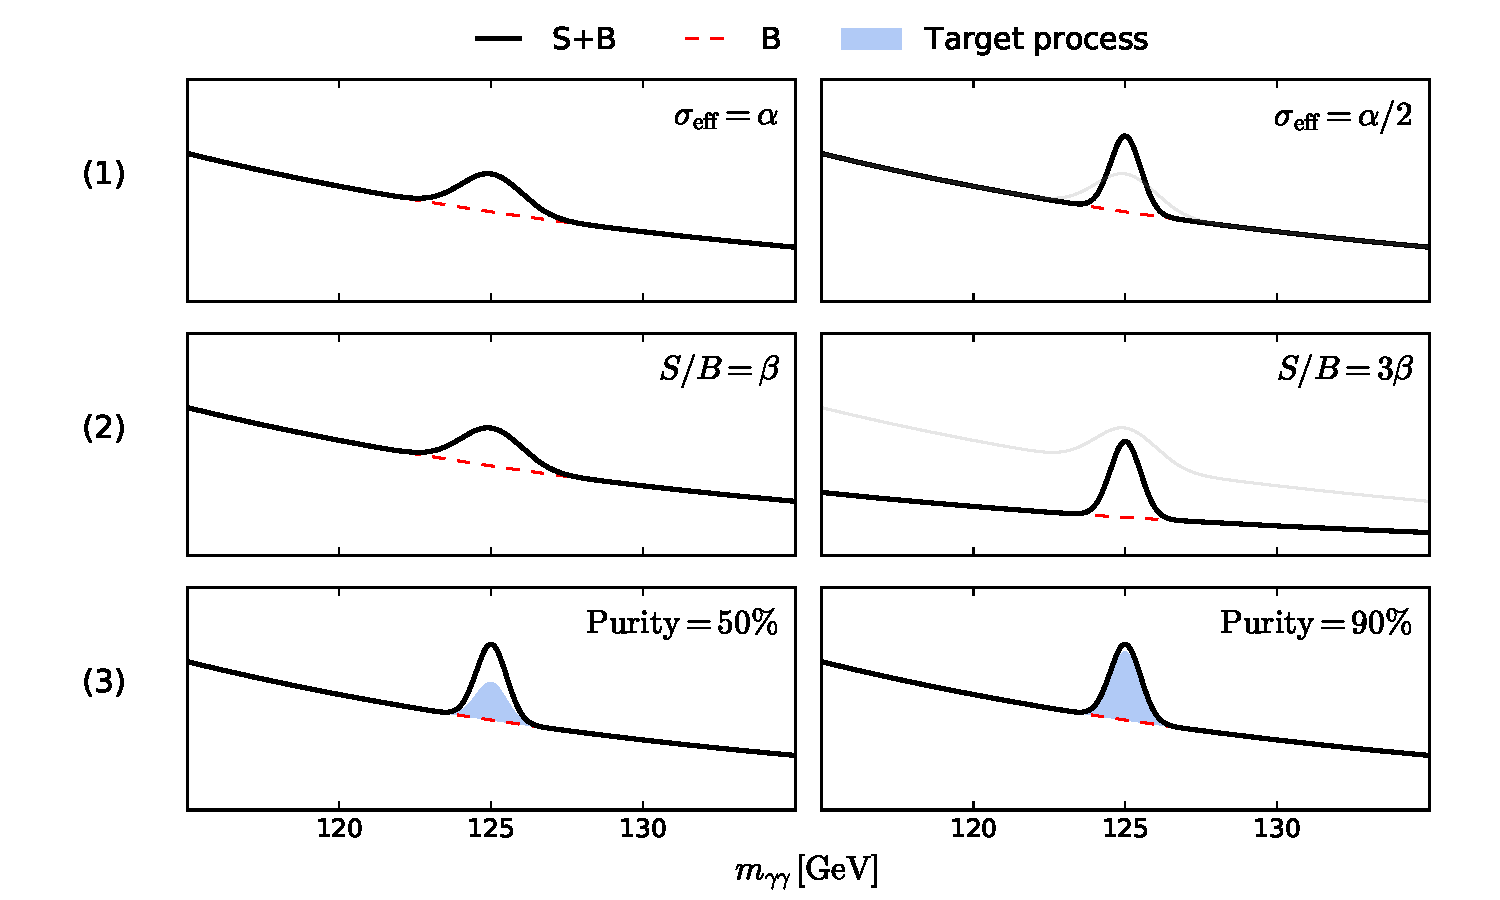
\includegraphics[width=1\textwidth]{Figures/hgg_overview/hgg_improve_measurement.pdf}
  \caption[Avenues for improving \Hgg measurements.]
  {
    Detailed caption
  }
  \label{fig:hgg_overview_improving_measurements}
\end{figure}

This chapter will focus on the experimental techniques used to maximise the sensitivity of the analysis, according to the three aspects stated above. After first introducing the data and simulation samples used in the analysis, section \ref{sec:event_reconstruction} details the procedure used to reconstruct candidate \Hgg events, specifically the techniques which improve the diphoton mass resolution, namely the photon identification and selection, the photon energy regression and the primary vertex selection. Following this, the categorisation of events is described in section~\ref{sec:event_categorisation}. Additional objects in the events such as jets, charged leptons and missing transverse momentum are used to define categories targeting the different STXS stage 1.2 bins. This section covers the methods used to both reduce background contamination and to increase the purity of the targeted signal process in such categories.

\section{Samples}
\subsection{Data}
This analysis uses p-p collision data collected by the CMS experiment at $\sqrt{s}$~=~13~TeV during Run 2 of the LHC. The total integrated luminosity is 137~\fbinv, of which 35.9~\fbinv was collected in 2016, 41.5~\fbinv in 2017 and 59.4~\fbinv in 2018.

Events in data are selected using the two-tiered trigger system described in section \ref{sec:trigger}. A seed at the L1T stage is defined as a deposit of energy in the ECAL, above a certain energy threshold, which is subsequently passed to the HLT path. Despite signal events being characterised by two photon candidates, a higher overall efficiency is achieved if only one seed is required at the L1T stage, with a tight transverse energy threshold applied to the seed in order to limit the rate of events passing to a manageable level. The energy threshold is typically set at 40~GeV, lowering to 30-32~GeV for isolated L1T seeds in the ECAL. With the presence of this energy threshold, there is an unavoidable drop in efficiency for \Hgg events at low transverse energy. To circumvent this effect, an additional double-seed selection is included at the L1T with lower energy thresholds than the single-seed trigger. In 2016, the thresholds were set to 23 and 10~GeV for the leading and subleading seeds respectively, rising to 25 and 14~GeV for the 2017 and 2018 data taking periods.

At the HLT, a basic version of the offline clustering algorithm, described in section \ref{sec:particle_flow}, is applied to the energy deposits in the ECAL. Here, events are required to contain two SCs with invariant mass greater than 90~GeV and passing asymmetric $p_T$ thresholds, initially set at 30 and 18~GeV. After the 2016 data-taking period, the lower threshold was raised to 22~GeV to counterbalance the increased instantaneous luminosity and hence maintain a constant event rate. In addition, a number of selection criteria are imposed on higher-level variables related to the SC shower shape, isolation and the ratio of the HCAL and ECAL deposits. Events passing the HLT selection then enter the \Hgg analysis.

The tag-and-probe method is used to evaluate the efficiency of the trigger selection~\cite{CMS:2011aa}. This method exploits the decay of a known resonance such as the $J/\psi$ or Z boson, where the \textit{tag} is defined as one of the decay products passing very tight identification criteria, and the \textit{probe} as the other decay product, subject to much looser identification requirements. Moreover, the combined invariant mass of the tag-and-probe pair is required to be consistent with the mass of the original resonance to ensure a high purity sample. For some selection criteria, $\mathcal{C}$, the efficiency, $\epsilon_{\mathcal{C}}$, is then defined as the fraction of probes passing $\mathcal{C}$. This method remains valid as long as the identification requirements on the probe do not affect the efficiency of $\mathcal{C}$.

Given the proximity of the Z boson and Higgs boson masses, as well as the fact that both electrons and photons are reconstructed as SCs in the ECAL, \Zee events in data provide an excellent candidate for evaluating efficiencies in the \Hgg analysis. Dielectrons with invariant mass close to the Z boson mass are used to define the tag and probe. After reweighting the \Zee events to match the $\eta$ and $R_9$ (see section \ref{sec:photon_preselection}) distributions of \Hgg events, the trigger efficiency is evaluated per SC in bins of the probe electron $p_T$, $\eta$ and $R_9$. For photons in the EB and EE, the trigger efficiency is above XX and YY\% respectively. The product of the two per-SC efficiencies is then used to weight simulated events to replicate the trigger efficiency observed in data.

\subsection{Simulation}
Monte Carlo (MC) simulated events are used for both training event classifiers and constructing the final signal model. 

Signal samples are simulated for the different Higgs boson production mechanisms at next-to-leading order (NLO) in quantum chromodynamics (QCD) using the \textsc{MG5\_aMC@NLO} (version 2.4.2)~\cite{}, and \textsc{Powheg} (version 2.0) generators~\cite{}. When possible, an independent event sample from the alternative generator is used for training event classifiers, thus ensuring the event categorisation and the construction of the final signal model are independent. Events produced via ggH production are weighted as a function of $p_T$ and $\eta$ to match the predictions of the NNLOPS program~\cite{}. Parton distribution functions (PDFs) are used to model the distribution of colliding partons inside the initial state protons. Events are subsequently interfaced with \textsc{Pythia8} (version 8.226 for 2016 MC and version 8.230 for 2017/2018 MC) for decaying the Higgs boson to photons, parton showering and hadronization~\cite{}. 

The signal samples are normalised according to the production cross sections and the \Hgg branching fraction (0.227\%) recommendations by the LHCHWG~\cite{}. The fractional breakdown of each production mode in the STXS stage 1.2 bins is computed directly from the signal MC samples, and serves as the SM prediction of the cross section in each bin. Table \ref{tab:signal_samples} summarises the event generators, PDF sets and \textsc{Pythia} tunes used for the signal simulation, as well as the total cross section times branching ratio for each production mode with details on the order of the calculation. The fractional breakdowns of each production mode into the stage 1.2 bins are shown in Tables~\ref{tab:stxs_frac_ggH}--\ref{tab:stxs_frac_top}.

\begin{table}[htb]
    \caption{Add caption: cross section evaluated at 13 TeV + MH. Actually fill table in correctly}
    \label{tab:signal samples}
    \vspace{.5cm}
    \centering
    \centering
    \scriptsize
    \renewcommand{\arraystretch}{1.8}
    \begin{tabular}{lccccc}
       & Generator (for classifiers) & \textsc{PYTHIA8} tune & PDF & $\sigma\cdot\rm{BR}$~[fb] & Order of $\sigma$ calc \\ \hline
       ggH & \textsc{Madgraph5\_aMC@NLO} & \textsc{Pythia8} & - & 110.27 & N$^{\rm{3}}$LO(QCD)+NLO(EW) \\
       gg$\rightarrow$ZH, Z$\rightarrow$qq & \textsc{Powheg} & \textsc{Pythia8} & - & 0.19 & NNLO(QCD)+NLO(EW) \\
       \hline
       VBF & \textsc{Madgraph5\_aMC@NLO} & \textsc{Pythia8} & - & 8.59 & NNLO(QCD)+NLO(EW) \\
       qq/qg$\rightarrow$WH, W$\rightarrow$qq & \textsc{Madgraph5\_aMC@NLO} & \textsc{Pythia8} & - & 2.10 & NNLO(QCD)+NLO(EW) \\
       qq/qg$\rightarrow$ZH, Z$\rightarrow$qq & \textsc{Madgraph5\_aMC@NLO} & \textsc{Pythia8} & - & 1.40 & NNLO(QCD)+NLO(EW) \\
       \hline
       qq/qg$\rightarrow$WH, W$\rightarrow\ell\nu$ & \textsc{Madgraph5\_aMC@NLO} & \textsc{Pythia8} & - & 1.016 & NNLO(QCD)+NLO(EW) \\
       qq/qg$\rightarrow$ZH, Z$\rightarrow\ell\ell/\nu\nu$ & \textsc{Madgraph5\_aMC@NLO} & \textsc{Pythia8} & - & 0.520 & NNLO(QCD)+NLO(EW) \\
       gg$\rightarrow$ZH, Z$\rightarrow\ell\ell/\nu\nu$ & \textsc{Powheg} & \textsc{Pythia8} & - & 0.084 & NNLO(QCD)+NLO(EW) \\
       \hline
       ttH & \textsc{MG5\_aMC@NLO} & \textsc{Pythia8} & - & 1.155 & NLO(QCD)+NLO(EW) \\
       \hline
       tHq & \textsc{MG5\_aMC@NLO} & \textsc{Pythia8} & - & 0.175 & NLO(QCD) in 5FS \\
       tHW & \textsc{MG5\_aMC@NLO} & \textsc{Pythia8} & - & 0.034 & NLO(QCD) in 5FS \\
       \hline
       bbH & \textsc{MG5\_aMC@NLO} & \textsc{Pythia8} & - & 1.108 & NNLO(5FS)+NLO(4FS) \\

    \end{tabular}
\end{table}

The final background model used for the extraction of results is derived directly from data. Nevertheless, simulated background events are required for training the multivariate event classifiers. For inclusive production, the dominant source of background is SM diphoton production, which is simulated using the \textsc{sherpa} (version 2.2.4) generator~\cite{}. In this sample, matrix elements are calculated at NLO and LO for up to one and up to three additional partons respectively, which are subsequently matched with the \textsc{Sherpa} generator parton showering. A subdominant background originates from $\gamma$~+~jet or jet~+~jet events, where the jets are misidentified as photons. These backgrounds are simulated with \textsc{Pythia8}, applying a filter in the generation to enrich the production of jets with high electromagnetic activity. Furthermore, other sources of background become important for categories targeting the sub-dominant production modes, such as $V+\gamma\gamma$ in the VH leptonic categories and $tt+\gamma\gamma$ in the top-associated categories. Additional MC samples simulated with the XYZ are used to model such backgrounds.

Finally, Drell-Yan events with leptonic final states are used for validation purposes and are simulated with the \textsc{MG5\_aMC@NLO} generator.

Each sample is propagated through the \textsc{Geant4} package to model the response of the CMS detector~\cite{}. Separate MC samples are produced for each year to account for the variations in the detector conditions and the LHC beam parameters. This modelling includes the effect of pileup interactions originating from both the nominal bunch cross-crossing (in-time pileup) and the crossing of previous and subsequent bunch crossings (out-of-time pileup). The simulation is weighted to match the distribution of the number of interaction vertices in data, which corresponds to an average pileup of 23 in 2016, and 32 in 2017 and 2018.

\section{Event reconstruction}\label{sec:event_reconstruction}
This section describes the offline reconstruction of events passing the trigger selection. 


\subsection{Photon reconstruction}
Photons are defined using the set of photon candidates from the PF algorithm (see section \ref{sec:particle_flow}). In the algorithm, SC's are formed by clustering together deposits of energy in the ECAL crystals, consistent with originating from the same electromagnetic shower. Due to imperfect shower containment in the crystals and shower losses for photons which convert to \ee pairs before reaching the ECAL, the SC energy, \Eraw, can often differ from the true initial photon energy, \Etrue. A multivariate regression technique is used to correct for such losses per photon, estimating both \Etrue and its uncertainty. Remaining differences in the photon energy scale and resolution are accounted for using a series of additional scale and smearing corrections, derived using \Zee events. Photons are then subject to a set of selection criteria (pre-selection) concerning the photon shower shape, kinematic and isolation variables. In addition, a photon identification Boosted Decision Tree (BDT) is trained to separate genuine photons from fake photons. The selection includes a minimum requirement on the output score of this BDT to vastly reduce the contribution from background processes entering the analysis, in which hadronic jets mimic the photon signature. Before describing the photon reconstruction techniques in more detail, it is useful to list the photon variables used in \Hgg analysis.

\subsubsection{Photon variables}

\subsubsection{Photon energy}
The photon energy response of the ECAL (\Etrue/\Eraw) is parameterised by a function with a Gaussian core and power law tails. Using simulated photons, a multivariate regressor is trained to estimate the shape parameters of this energy response function, thus providing a prediction of the full \Etrue/\Eraw probability density function for each photon~\cite{}. The mode of this predicted function is used to correct \Eraw to \Etrue, whilst the shape provides a per-photon energy resolution estimate used later in the event categorisation (section \ref{sec:event_categorisation}).

The regressor aims to correct not only for the imperfect shower containment arising from converting photons and electromagnetic showers that begin upstream of the ECAL, but also for the localised containment within the ECAL, where energy can be lost in the gaps between crystals. Input variables related to the SC shower shape provide information on the upstream showering and photon conversions, which combined with the SC $\eta$ and $\phi$ values allows the regressor to learn variations in the ECAL geometry. On the other hand, the seed crystal positions and seed cluster energy ratios enable the regressor to correct for the localised containment effects. In addition, the total number of primary vertices and the total energy density, $\rho$, are included to account for systematic enhancements of \Eraw due to pileup.

After the regression, a number of residual discrepancies between data and simulation remain, that cannot be derived from simulation alone. Using \Zee events in data, in which the electrons are reconstructed as photons, a series of scale and smearing corrections are derived to correct the photon energy scale and resolution~\cite{}. To account for the degradation of the ECAL crystal performance over time, and the subsequent drift in energy scale this would cause, a time-dependent correction is applied in bins which equate roughly to the duration of one LHC fill. This ensures the energy scale of the ECAL is constant over time. Subsequently, the dielectron mass spectrum, $m_{ee}$, is used to simultaneously shift the peak in data to match that in simulation, and smear the resolution in simulation to match that in data. These scale and smearing corrections are applied differentially in bins of SC $\eta$ and \RNINE. 

Referring back to equation \ref{eq:mgg}, the techniques described above aim to minimize the photon energy resolution, $\sigma_E/E$, in turn minimizing the diphoton mass resolution, $\sigma_m/m_{\gamma\gamma}$, and thus leading to an enhanced sensitivity to Higgs boson production. Figure \ref{fig:photon_energy_0} shows the $m_{ee}$ distributions for \Zee events in both data and simulation, after the full set of energy corrections are applied. The left-hand panel shows the situation where both electrons are reconstructed in the ECAL barrel, and the right-hand panel where both are reconstructed in the ECAL endcaps. Clearly, after the corrections are applied, the data and simulation are in excellent agreement, well within the uncertainties.

\begin{figure}[hptb]
  \centering
  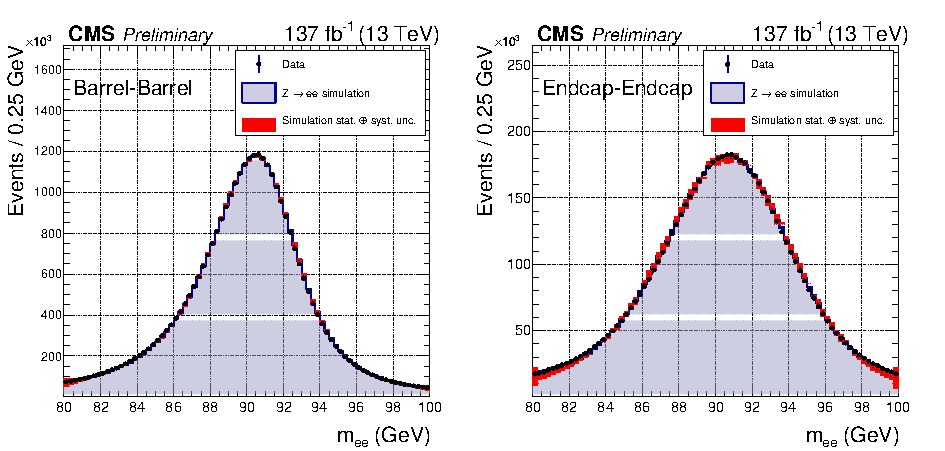
\includegraphics[width=1\textwidth]{Figures/hgg_overview/photon_energy_0.pdf}
  \caption[Dielectron mass spectrum for \Zee events in data and simulation after the energy corrections are applied]
  {
    Comparison of the dielectron mass spectrum for \Zee events in data (black points) and simulation (filled histogram), after the full set of energy scale and smearing corrections are applied. The total uncertainty on simulated events is shown by the red bands. The plots show the full data set collected during run II of the LHC, and the corresponding simulation, where the left-hand (right-hand) panel corresponds to events in which both electrons are reconstructed in the ECAL barrel (endcaps).
  }
  \label{fig:photon_energy_0}
\end{figure}

\subsubsection{Photon pre-selection}\label{sec:photon_preselection}
Table \ref{tab:photon_preselection} provides a schema of the selection criteria applied to the photon candidates. The pre-selection efficiency is calculated using the tag-and-probe method on \Zee events for all selection criteria, barring the requirement on the electron veto, which is computed using the photon in \Zmumug events. These efficiencies are computed for both data and simulation in bins of $\eta$ and \RNINE, and are typically above 95\% for photons with high values of \RNINE ($>0.85$) and around 90\% for photons with lower \RNINE ($<0.85$). The pre-selection efficiencies in simulation are scaled to match those in data.

\begin{table}[htb]
    \caption[Schema of the photon pre-selection criteria]{Schema of the photon pre-selection criteria. The shower shape and isolation requirements are different for photons in the ECAL barrel and for photons in the ECAL endcaps. These are then split into regions of different \RNINE criteria, with varying levels of additional selection on $\sigma_{\eta\eta}$, $\mathcal{I}_{\rm{ph}}$ and $\mathcal{I}_{\rm{tk}}$.}
    \label{tab:photon_preselection}
    \vspace{.5cm}
    \centering
    \scriptsize
    \renewcommand{\arraystretch}{1.5}
    \begin{tabular}{p{0.25\textwidth}|p{0.7\textwidth}}
       Minimum \pt  & $p_T^{\gamma 1}>35$~GeV (leading), $p_T^{\gamma 2}>25$~GeV (subleading) \\
       $\downarrow$ & \\
       Geometrical acceptance & $|\eta| < 2.5$, excluding barrel-endcap transition region $1.44 < |\eta| < 1.57$ \\
       $\downarrow$ & \\
       Electron veto & True \\
       $\downarrow$ & \\
       Hadronic shower rejection & H/E~$<0.08$ \\
       $\downarrow$ & \\
       Shower shape and isolation requirements
       & For photons in the EB:
       \begin{tabular}{c|ccc}
            \RNINE & $\sigma_{\eta\eta}$ & $\mathcal{I}_{\rm{ph}}$ (GeV) & $\mathcal{I}_{\rm{tk}}$ (GeV) \\ \hline
            $>0.85$ & - & - & - \\
            $[0.50,0.85]$ & $<0.015$ & $<4.0$ & $<6.0$ \\
       \end{tabular} \\
       & \\
       & For photons in the EE:
       \begin{tabular}{c|ccc}
            \RNINE & $\sigma_{\eta\eta}$ & $\mathcal{I}_{\rm{ph}}$ (GeV) & $\mathcal{I}_{\rm{tk}}$ (GeV) \\ \hline
            $>0.90$ & - & - & - \\
            $[0.80,0.90]$ & $<0.035$ & $<4.0$ & $<6.0$ \\
       \end{tabular} \\
       & \\
       & All photons: (\RNINE$>0.8$ and $\mathcal{I}_{\rm{ch}}<20$~GeV) or ($\mathcal{I}_{\rm{ch}}/p_T^{\gamma}<0.3$)

    \end{tabular}
\end{table}


\subsubsection{Photon identification}
The photon identification BDT aims to distinguish between real photons in the CMS detector and hadronic jets mimicking a photon signature. The BDT is trained using the $\gamma$~+~jet simulation sample, where the true photon is used as signal and the jet as background. Photon shower shape, kinematic and isolation variables are used as inputs to the BDT, along with parameters sensitive to pileup, such as $\rho$.

One of the dominant sources of systematic uncertainty in the \Hgg analysis arises from the modeling of the electromagnetic shower in simulation, in particular the variables describing the shower shape and isolation. Since these variables are direct inputs to the photon identification BDT, any discrepancies between data and simulation are propagated to the output BDT score, and therefore introduce a systematic uncertainty into the analysis. To mitigate this, 

Output score distributions. Uses.

One of main systematic uncertainties. Chained quantile regression to ensure shower shape and isolation variables agree. Explain reduction in systematic uncertainty using this technique.


\subsection{Vertex selection}
Equation \ref{eq:mgg} demonstrates that the diphoton mass resolution depends not only on the per-photon energy resolutions, but also on the determination of the photon opening angle, $\theta$. For this, it is necessary to know the precise location of the primary hard-scattering vertex from which the photons originate. If the location is correctly determined within 1~cm of the true vertex position, the diphoton mass resolution is dominated by the photon energy resolution. For events with additional objects such as charged leptons and jets, it is relatively easy to assign the primary vertex, due to the presence of distinct charged particle tracks. On the other hand, for \Hgg events with no additional objects (e.g. ggH 0J), it becomes a much more difficult problem. In the \Hgg anaylsis, the diphoton vertex assignment is performed using a dedicated BDT, which is trained using ggH \Hgg simulated events and takes as input variables related to the tracks recoiling against the diphoton system:

\begin{itemize}
    \item $\sum_i |\vec{p}^{\,i}_T|^2$,
    \item $-\sum_i (\vec{p}^{\,i}_T\cdot \vec{p}_T^{\,\gamma\gamma}/|\vec{p}_T^{\,\gamma\gamma}|)$,
    \item $(|\sum_i \vec{p}^{\,i}_T| - p_T^{\,\gamma\gamma})/(|\sum_i \vec{p}^{\,i}_T| + p_T^{\,\gamma\gamma})$,
    \item the total number of photon conversions in the tracker,
    \item the pull ($|z_{\rm{vtx}}-z_{\rm{e}}|/\sigma_z$) between the longitudinal positions of the reconstructed vertex, $z_{\rm{vtx}}$ and the vertex estimated using tracks from photon conversions, $z_e$, where $\sigma_z$ is the uncertainty in $z_{\rm{e}}$,
\end{itemize}

\noindent
where the sum runs over all particle flow tracks associated with a given vertex, labelled by the index, $i$. The quantity $\vec{p}_T^{\,\gamma\gamma}$ corresponds to transverse momentum of the diphoton system, measured with respect to the same vertex. The final two BDT input variables in the list are only included for events which contain tracks originating from photon conversions. 

The performance of the vertex assignment BDT is evaluated using \Zmumu events. Here, the vertices are reconstructed after omitting the muon tracks, in order to imitate a diphoton-like system. The vertex is then said to be correctly assigned by the BDT if the location is within 1~cm of the true vertex position. Figure \ref{fig:vertex_selection_0} (left) shows the efficiency of the vertex assignment as a function of the dimuon $p_T$, for both simulation and data, demonstrating an agreement within 2\% across the whole $p_T$ range. Correction factors are applied to simulation to match the efficiencies observed in data, keeping the total number of events constant. For inclusive \Hgg events, the efficiency of correctly assigning the diphoton vertex to be within 1~cm of the true vertex is roughly 79\%. This value rises for events with additional objects such as jets and charged leptons.

An additional vertex-related BDT is trained to estimate the \textit{probability} that the vertex assignment is within 1~cm of the interaction point from which the diphoton originates. The inputs variables are the total number of reconstructed vertices in an event, the relative positions and respective vertex assignment BDT scores for the three highest scoring vertices, $|{p}_T^{\,\gamma\gamma}|$, as well as the number of converted photons in the tracker. Akin to the vertex-assignment BDT, this vertex-probability BDT is trained using ggH, \Hgg events. The right-hand panel of Figure \ref{fig:vertex_selection_0} demonstrates the agreement between the output probability and the vertex assignment efficiency for simulated \Zmumu events.

\begin{figure}[hptb]
  \centering
  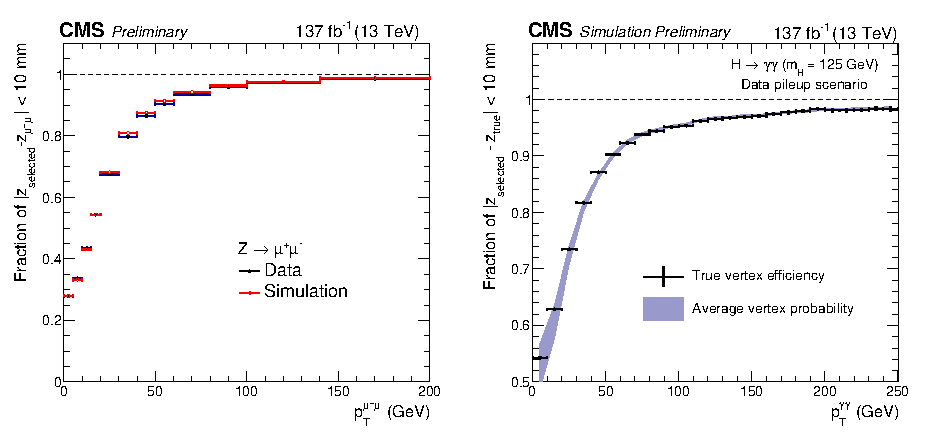
\includegraphics[width=1\textwidth]{Figures/hgg_overview/vertex_assignment_0.pdf}
  \caption[Vertex-assignment and vertex-probability BDT]
  {
    Add caption.
  }
  \label{fig:vertex_selection_0}
\end{figure}

Finally, the width of the $z$ distribution of reconstructed vertices, known as the beamspot width, is measured to be between 3.4--3.6~cm in data. A year-dependent correction is applied to simulated events to ensure the beamspot width matches that observed in data.

\subsection{Reconstruction of other objects}
Needed for categorisation.
\subsubsection{Jets}

\subsubsection{Electrons}

\subsubsection{Muons}

\subsubsection{Missing transverse momentum}



\section{Event categorisation}\label{sec:event_categorisation}

\subsection{Overview}
\begin{itemize}
    \item Merged across years: more statistics to train MVA
    \item Discuss tag sequence
    \item Briefly discuss Machine learning
    \item 
\end{itemize}

\subsection{Top associated production}

\subsection{VH leptonic production}

\subsection{qqH production}

\subsection{ggH production}

\subsection{Validation}

\subsection{Summary}
\begin{itemize}
    \item include purity and migration matrices
\end{itemize}



